\documentclass[conference]{IEEEtran}
\IEEEoverridecommandlockouts

\usepackage{cite}
\usepackage{amsmath,amssymb,amsfonts}
\usepackage{graphicx}
\usepackage{textcomp}
\usepackage{xcolor}
\usepackage{listings}
\usepackage{hyperref}
\usepackage{tikz}
\usetikzlibrary{positioning}
\usepackage{pgf-umlcd}
\usepackage{booktabs}
\usepackage{array}

% Code listing style for Go
\lstdefinelanguage{Go}{
  morekeywords={package,import,func,return,type,struct,interface,var,const,
                if,else,for,range,switch,case,default,break,continue,
                go,chan,select,defer,map,make,nil,true,false,append,len,cap,
                error,string,int,float64,bool},
  sensitive=true,
  morecomment=[l]{//},
  morecomment=[s]{/*}{*/},
  morestring=[b]",
}

\lstset{
  language=Go,
  basicstyle=\ttfamily\footnotesize,
  keywordstyle=\bfseries\color{blue!70!black},
  commentstyle=\itshape\color{green!50!black},
  stringstyle=\color{red!60!black},
  numbers=left,
  numberstyle=\tiny\color{gray},
  numbersep=5pt,
  breaklines=true,
  showstringspaces=false,
  frame=single,
  rulecolor=\color{gray!40},
  captionpos=b,
  tabsize=4,
  xleftmargin=1em,
}

\def\BibTeX{{\rm B\kern-.05em{\sc i\kern-.025em b}\kern-.08em
    T\kern-.1667em\lower.7ex\hbox{E}\kern-.125emX}}

\begin{document}

\title{Implementation of Factory, Strategy, and Facade Design Patterns in a Go-Based Cinema Ticket Booking REST API}

\author{
  \IEEEauthorblockN{Nandana Rajendra Kawiswara, Abid Farhan Abdullah, Octa Ramadhani Rinantoro,\\ Andra Al Ayubi, Andru Falah Arifin}
  \IEEEauthorblockA{
    \textit{Department of Informatics Engineering}\\
    \textit{Politeknik Elektronika Negeri Surabaya}\\
    Surabaya, Indonesia
  }
}

\maketitle

\begin{abstract}
Managing backend systems often leads to messy code when dealing with complex business workflows like cinema seat reservations and dynamic pricing. This paper shares our experience structuring a REST API called \textit{gin-M-TIX} using Go and the Gin framework. We integrated three design patterns to keep the codebase modular. The Factory Method pattern manages object generation across four ticket tiers (regular, VIP, and student options) using a double boolean check on user and seat data. The Strategy pattern handles time-sensitive pricing, shifting calculations out of the main service layer. Lastly, a Facade simplifies how the API endpoint handles booking and payment step sequences. We verified the architecture using integration tests, showing that separating these concerns keeps handlers clean and makes it easy to add new business rules without breaking existing routes or impacting performance.
\end{abstract}

\begin{IEEEkeywords}
design patterns, Factory Method, Strategy, Facade, Go, Gin framework, REST API, software architecture, cinema booking system
\end{IEEEkeywords}

% ─────────────────────────────────────────────
\section{Introduction}

In backend development, writing code that is easy to extend and debug is a major goal. As systems grow, adding new rules often results in nested conditionals that clutter core services. Software design patterns~\cite{gamma1994design} are standard ways to solve these architecture issues~\cite{alhawari2022patterns}. Most design pattern guides use traditional object-oriented languages like Java, leaving a gap in how to apply them cleanly to languages like Go. Go has no classes or inheritance, relying instead on composition and interfaces.

To study these patterns in a Go context, we built \textit{gin-M-TIX}, a backend service for booking cinema seats. It supports standard features like listing movies, checking schedules, allocating seats, processing bookings, and recording payments. Instead of putting all logic directly into the HTTP handler functions, we structured the API around three patterns: the Factory Method (creational), the Strategy (behavioral), and the Facade (structural).

Our work focus is to show how these patterns solve real-world problems in a web API. Rather than just repeating textbook definitions, we document:
\begin{itemize}
  \item How to use Go's implicit interfaces to write decoupling code without standard OOP boilerplates.
  \item A clean project layout that keeps patterns in separate folders to prevent import cycles.
  \item How the facade decouples the HTTP controllers from internal logic, making the code much easier to write tests for.
  \item The interaction between different pattern outputs, where the pricing strategy's base calculation directly feeds into the ticket creation factory.
\end{itemize}

The paper is structured as follows: Section~\ref{sec:background} looks at design pattern theory. Section~\ref{sec:system} presents the system structure. Sections~\ref{sec:factory} through \ref{sec:facade} explain the implementations. Section~\ref{sec:evaluation} discusses the code evaluation, and Section~\ref{sec:conclusion} concludes the paper.

% ─────────────────────────────────────────────
\section{Background and Related Work}
\label{sec:background}

\subsection{Design Patterns and Modern Web Systems}

Design patterns are reusable templates to solve software structure issues. The Gang of Four~\cite{gamma1994design} grouped these into three types: Creational, Structural, and Behavioral~\cite{flageol2023mapping}. In web development, developers frequently run into issues like bloated route handlers and hardcoded object logic. Applying these patterns helps isolate the HTTP routing layer from the actual business computations, keeping the code clean as requirements change.

\subsection{Go's Approach to Object-Oriented Design}

Go is not a traditional object-oriented language. It does not support class hierarchies or extends keywords. Instead, polymorphism is achieved through implicit interfaces, where a struct satisfies an interface simply by matching its methods~\cite{ozkaya2021despat}. This implicit nature is useful when implementing patterns like Strategy or Factory Method because developers do not need to write long inheritance chains. Structs can remain small and focused on a single responsibility.

\subsection{Structuring REST APIs in Go}

Web backends need to handle incoming HTTP requests quickly and safely. Go's Gin framework~\cite{gin2024} provides fast routing with minimal overhead, but it does not prescribe a specific codebase layout. Without design patterns, developers often place database queries, request validation, and business logic inside the same controller functions. This makes the code difficult to unit test. By combining Gin with structured patterns, we can mock database structures and test the system rules independently~\cite{golmohammadi2022testing}.

% ─────────────────────────────────────────────
\section{System Architecture}
\label{sec:system}

\subsection{Project Structure}

We organized \textit{gin-M-TIX} into a layered layout to keep database models, SQL-like queries, business rules, and HTTP endpoints in separate packages. The design patterns are grouped inside a folder named \texttt{patterns/} to keep them separate from the main services.

{\footnotesize
\begin{verbatim}
gin-M-TIX/
|-- main.go
|-- config/       # Database mock setup
|-- controllers/  # API route handlers
|-- models/       # Data structures
|-- repositories/ # Storage queries
|-- services/     # Service controllers
|-- patterns/
|   |-- factory/  # Ticket factory
|   |-- strategy/ # Pricing strategy
|   \-- facade/   # Booking facade
\-- routes/       # Router mappings
\end{verbatim}
}

\subsection{Data Processing Flow}

When a client sends a request to book a seat, the data flows through the layers like this:

\begin{enumerate}
  \item \texttt{BookingController} reads the JSON payload from the client.
  \item It passes the parameters directly to the \texttt{BookingFacade}.
  \item The facade calls the \texttt{BookingService}, which coordinates with the \texttt{PricingService}.
  \item The \texttt{PricingService} runs the active \texttt{PricingStrategy} to calculate base costs.
  \item The service uses the calculated base price and calls \texttt{NewTicketFactory} to build the ticket structures.
  \item The results are written to the database using the repository classes.
\end{enumerate}

\subsection{Mock Database Implementation}

Instead of setting up an external database like MySQL or PostgreSQL, we wrote a simple \texttt{config.Database} struct that holds lists of movies, studios, seats, schedules, and bookings in memory. This setup makes it easy to run and test the application without any external configuration.

% ─────────────────────────────────────────────
\section{Factory Method Pattern}
\label{sec:factory}

\subsection{Intent and Motivation}

The Factory Method pattern defines an interface for creating objects but allows the system to choose the exact struct type at runtime~\cite{gamma1994design}. In our application, we support regular and VIP seats, and offer discounts for student users. If we wrote this logic using nested \texttt{if-else} statements inside the main booking loop, the booking service would become tightly coupled to individual ticket properties. We used the Factory Method to separate this creation logic, ensuring the service layer only interacts with a generic \texttt{TicketFactory} interface.

\subsection{Key Components}

\begin{itemize}
  \item \textbf{Product Struct}: \texttt{models.Ticket} --- holds details like seat code, type, and final price.
  \item \textbf{Creator Interface}: \texttt{TicketFactory} --- declares the \texttt{CreateTicket()} method.
  \item \textbf{Concrete Creators}: \texttt{RegularTicketFactory}, \texttt{VIPTicketFactory}, \texttt{RegularStudent}\-\texttt{TicketFactory}, and \texttt{VIPStudent}\-\texttt{TicketFactory}.
  \item \textbf{Selector Function}: \texttt{NewTicketFactory(isVIP, isStudent bool)} --- determines the correct struct to return using two boolean flags.
\end{itemize}

\subsection{Mathematical Model and Class Diagram}

We calculate ticket prices based on seat type and student status. Let $P_{base}$ represent the base price (after showtime calculations). Let $v \in \{0, 1\}$ represent whether a seat is VIP, and let $s \in \{0, 1\}$ indicate student status. The final price $P_{ticket}$ is:

\begin{equation}
P_{ticket}(v, s) =
\begin{cases}
P_{base} \times 1.5 \times 0.8 & \text{for } v = 1, s = 1 \\
P_{base} \times 1.5 & \text{for } v = 1, s = 0 \\
P_{base} \times 0.8 & \text{for } v = 0, s = 1 \\
P_{base} & \text{for } v = 0, s = 0
\end{cases}
\end{equation}

Figure~\ref{fig:factory_diagram} outlines how the creator classes implement the common factory interface.

\begin{figure}[htbp]
\centering
\resizebox{\linewidth}{!}{
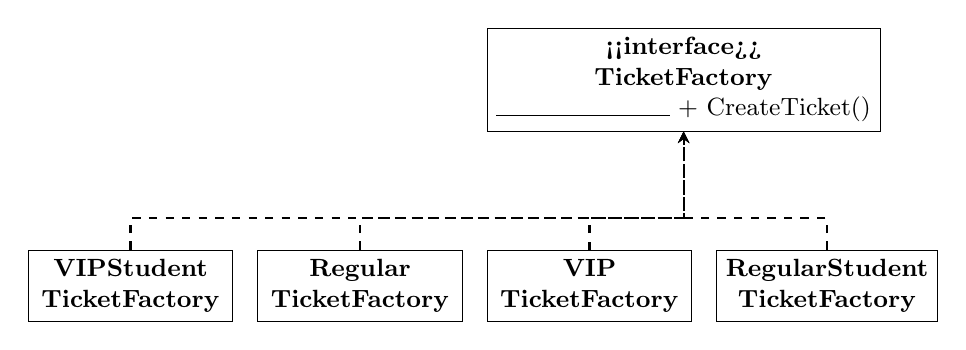
\begin{tikzpicture}[
  node distance=1.2cm and 0.3cm,
  box/.style={draw, rectangle, minimum width=2.6cm, minimum height=0.9cm, align=center, font=\small},
  arrow/.style={-stealth, dashed, thick}
]
\node[box] (factory) {\textbf{<<interface>>} \\ \textbf{TicketFactory} \\ \rule{2.2cm}{0.4pt} + CreateTicket()};
\node[box, below left=1.5cm and 0.3cm of factory] (regular) {\textbf{Regular} \\ \textbf{TicketFactory}};
\node[box, left=of regular] (vipstudent) {\textbf{VIPStudent} \\ \textbf{TicketFactory}};
\node[box, right=of regular] (vip) {\textbf{VIP} \\ \textbf{TicketFactory}};
\node[box, right=of vip] (regstudent) {\textbf{RegularStudent} \\ \textbf{TicketFactory}};

\draw[arrow] (vipstudent.north) -- ++(0,0.4) -| (factory.south);
\draw[arrow] (regular.north) -- ++(0,0.4) -| (factory.south);
\draw[arrow] (vip.north) -- ++(0,0.4) -| (factory.south);
\draw[arrow] (regstudent.north) -- ++(0,0.4) -| (factory.south);
\end{tikzpicture}
}
\caption{UML Class Diagram of the Ticket Factory Pattern}
\label{fig:factory_diagram}
\end{figure}

\subsection{Integrating the Factory}

Inside \texttt{BookingService}, ticket instantiation is handled cleanly. For each seat in the booking request, the service runs \texttt{NewTicketFactory(seat.IsVIP, isStudent)}. This returns a struct that satisfies the \texttt{TicketFactory} interface. The service calls \texttt{CreateTicket()} without needing to know which subclass is doing the work or what specific math rules apply.

\subsection{Summary of Multipliers}

Table~\ref{tab:ticket_types} shows the pricing rules for each ticket struct.

\begin{table}[htbp]
\caption{Ticket Type Modifiers}
\label{tab:ticket_types}
\begin{center}
\begin{tabular}{p{1.6cm}p{2.8cm}p{2.2cm}}
\toprule
\textbf{Type} & \textbf{Factory Struct} & \textbf{Multiplier} \\
\midrule
regular          & RegularTicketFactory        & $\times 1.0$ \\
vip              & VIPTicketFactory            & $\times 1.5$ \\
regular\_student & RegularStudentTicketFactory & $\times 0.8$ \\
vip\_student     & VIPStudentTicketFactory     & $\times 1.5 \times 0.8$ \\
\bottomrule
\end{tabular}
\end{center}
\end{table}

\subsection{Extensibility}

If we decide to add a new category, such as a senior citizen discount, we only need to write a new struct that implements the \texttt{TicketFactory} interface and add a condition check in \texttt{NewTicketFactory}. The main code inside \texttt{BookingService} does not change, keeping the application easy to expand.

% ─────────────────────────────────────────────
\section{Strategy Pattern}
\label{sec:strategy}

\subsection{Intent and Motivation}

The Strategy pattern defines a family of algorithms, encapsulating each one so they can be swapped easily~\cite{gamma1994design}. In our application, cinema ticket prices change depending on the day and time of the movie schedule. To avoid cluttering the pricing system with hardcoded time checks, we implemented separate pricing strategies. This design lets us add or adjust pricing policies without modifying the central transaction codes.

\subsection{Key Components}

\begin{itemize}
  \item \textbf{Strategy Interface}: \texttt{PricingStrategy} --- defines \texttt{Calculate()} and \texttt{Name()} methods.
  \item \textbf{Concrete Strategies}: \texttt{WeekdayPricing}, \texttt{WeekendPricing}, \texttt{MidnightPricing}, and \texttt{HolidayPricing}.
  \item \textbf{Context Class}: \texttt{PricingService} --- evaluates the schedule and applies the matching strategy.
\end{itemize}

\subsection{Pricing Model}

We write the pricing calculations inside separate strategy rules. Let $P_{base}$ be the standard base price of the schedule, and let $T$ represent the date or time. The pricing function $S(T)$ adjusts the rate as follows:

\begin{equation}
S(T) =
\begin{cases}
1.50 \times P_{base} & \text{Holiday } T \\
1.20 \times P_{base} & \text{Midnight } T \\
1.25 \times P_{base} & \text{Weekend } T \\
1.00 \times P_{base} & \text{Weekday (default)}
\end{cases}
\end{equation}

\subsection{Selection Logic and Structure}

The system processes rules based on priority. For example, a Holiday rule overrides the Weekend modifier if a holiday falls on a Saturday. Figure~\ref{fig:strategy_diagram} shows the structure of our strategy implementation.

\begin{figure}[htbp]
\centering
\resizebox{\linewidth}{!}{
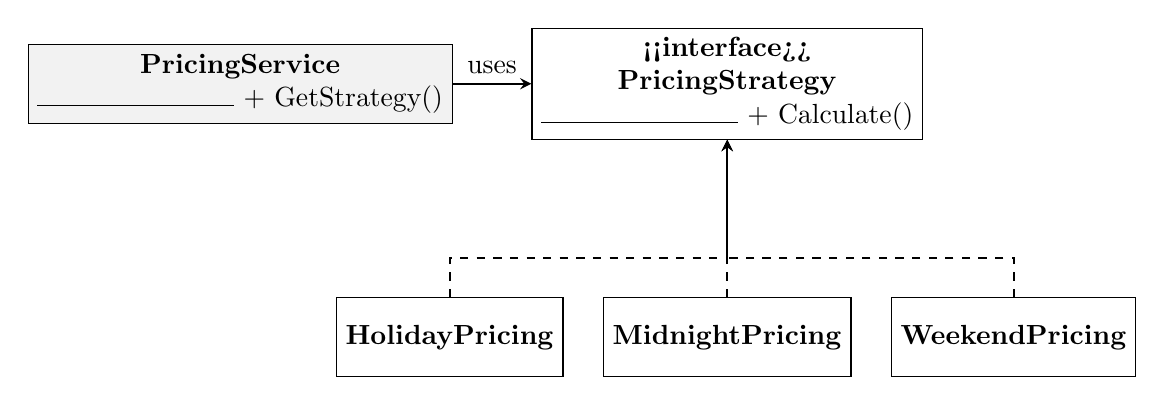
\begin{tikzpicture}[
  node distance=1.5cm and 0.5cm,
  box/.style={draw, rectangle, minimum width=2.8cm, minimum height=1cm, align=center},
  ctx/.style={draw, rectangle, minimum width=3cm, minimum height=1cm, align=center, fill=gray!10},
  arrow/.style={-stealth, dashed, thick},
  solidarrow/.style={-stealth, thick}
]
\node[box] (strategy) {\textbf{<<interface>>} \\ \textbf{PricingStrategy} \\ \rule{2.5cm}{0.4pt} + Calculate()};
\node[ctx, left=1cm of strategy] (context) {\textbf{PricingService} \\ \rule{2.5cm}{0.4pt} + GetStrategy()};

\node[box, below=of strategy, yshift=-0.5cm] (mid) {\textbf{MidnightPricing}};
\node[box, left=of mid] (hol) {\textbf{HolidayPricing}};
\node[box, right=of mid] (week) {\textbf{WeekendPricing}};

\draw[solidarrow] (context) -- (strategy) node[midway, above] {uses};
\draw[arrow] (hol.north) -- ++(0,0.5) -| (strategy.south);
\draw[arrow] (mid.north) -- (strategy.south);
\draw[arrow] (week.north) -- ++(0,0.5) -| (strategy.south);
\end{tikzpicture}
}
\caption{UML Class Diagram of the Strategy Pattern}
\label{fig:strategy_diagram}
\end{figure}

\subsection{Strategy Settings}

Table~\ref{tab:strategies} outlines the triggers for each strategy.

\begin{table}[htbp]
\caption{Pricing Rules and Triggers}
\label{tab:strategies}
\begin{center}
\begin{tabular}{p{1.5cm}p{3.5cm}p{1.8cm}}
\toprule
\textbf{Strategy} & \textbf{Condition} & \textbf{Multiplier} \\
\midrule
Holiday   & Jan 1 or Dec 25             & $\times 1.5$ \\
Midnight  & Hour $\geq$ 22 or $\leq$ 2  & $\times 1.2$ \\
Weekend   & Saturday or Sunday          & $\times 1.25$ \\
Weekday   & All other times             & $\times 1.0$ \\
\bottomrule
\end{tabular}
\end{center}
\end{table}

\subsection{Adding Strategies}

If we want to add a promotional rate, we do not need to rewrite the main booking code. We write a new struct that satisfies the \texttt{PricingStrategy} interface and add a condition check inside \texttt{GetStrategy}.

% ─────────────────────────────────────────────
\section{Facade Pattern}
\label{sec:facade}

\subsection{Intent and Motivation}

The Facade pattern provides a simplified interface to a complex set of classes in a subsystem~\cite{gamma1994design}. In our cinema API, booking a ticket requires coordinating two distinct backend modules: the \texttt{BookingService} (reserving seats and creating tickets) and the \texttt{PaymentService} (checking funds and finalizing transactions). If the HTTP controller interacted with these modules directly, it would contain excessive orchestrating code. By introducing the Facade pattern, we provide a single entry point that simplifies controllers and hides subsystem coordination.

\subsection{Key Components}

\begin{itemize}
  \item \textbf{Facade Class}: \texttt{BookingFacade} --- coordinates booking and payment service classes.
  \item \textbf{Subsystems}: \texttt{BookingService} and \texttt{PaymentService}.
  \item \textbf{Client Class}: \texttt{BookingController}.
\end{itemize}

\subsection{Architecture Design}

Figure~\ref{fig:facade_diagram} shows how the facade acts as a clean gateway, isolating the controller from the specific backend service classes.

\begin{figure}[htbp]
\centering
\resizebox{\linewidth}{!}{
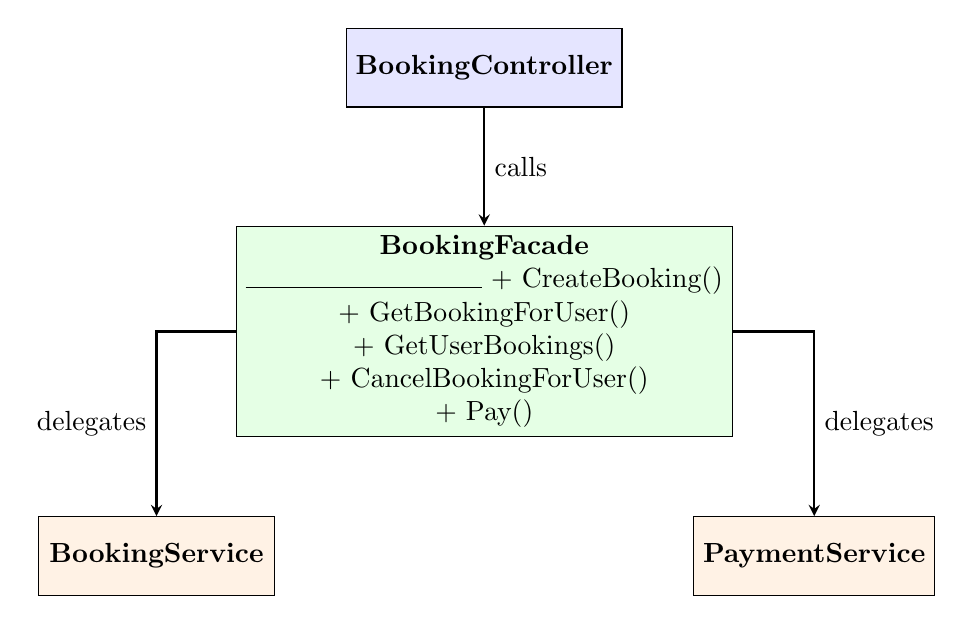
\begin{tikzpicture}[
  node distance=1.5cm and 1cm,
  client/.style={draw, rectangle, minimum width=3cm, minimum height=1cm, align=center, fill=blue!10},
  facade/.style={draw, rectangle, minimum width=4cm, minimum height=1cm, align=center, fill=green!10},
  svc/.style={draw, rectangle, minimum width=3cm, minimum height=1cm, align=center, fill=orange!10},
  arrow/.style={-stealth, thick}
]
\node[client] (ctrl) {\textbf{BookingController}};
\node[facade, below=of ctrl] (facade) {\textbf{BookingFacade} \\ \rule{3cm}{0.4pt} + CreateBooking() \\ + GetBookingForUser() \\ + GetUserBookings() \\ + CancelBookingForUser() \\ + Pay()};
\node[svc, below left=1cm and -0.5cm of facade] (bookSvc) {\textbf{BookingService}};
\node[svc, below right=1cm and -0.5cm of facade] (paySvc) {\textbf{PaymentService}};

\draw[arrow] (ctrl) -- (facade) node[midway, right] {calls};
\draw[arrow] (facade) -| (bookSvc) node[pos=0.75, left] {delegates};
\draw[arrow] (facade) -| (paySvc) node[pos=0.75, right] {delegates};
\end{tikzpicture}
}
\caption{Architecture Diagram of the Facade Pattern}
\label{fig:facade_diagram}
\end{figure}

\subsection{Simplifying API Handlers}

With the facade pattern, the controller is only responsible for parsing HTTP JSON requests and returning status codes. It does not handle validation rules or coordinate steps, which keeps the handler functions clean and readable.

% ─────────────────────────────────────────────
\section{Evaluation and Discussion}
\label{sec:evaluation}

\subsection{Package Dependency and Circular Imports}

A common issue in Go projects is circular dependencies. When packages import each other, the Go compiler throws an error and stops the build. 

By grouping our design patterns into the \texttt{patterns/} package, we avoided circular imports. Structs in \texttt{patterns/factory} and \texttt{patterns/strategy} do not import any logic classes; they only import the basic data definitions in \texttt{models}. The main logic classes in \texttt{services/} import \texttt{patterns/}, but the reverse is not true. This unidirectional import layout ensures that our code compiles without issues and maintains clean boundaries.

\subsection{Extensibility Test Cases}

To evaluate how easily our architecture can be modified, we analyzed the change requirements for adding new features. 

For example, to add a new ticket category like a senior discount, we do not need to modify the controller or the main \texttt{BookingService} class. We only have to write a single struct implementing \texttt{TicketFactory} and add its selection check in \texttt{NewTicketFactory}. We verified this extensibility using integration tests in \texttt{routes\_test.go}, specifically checking the pricing rules for student discounts and VIP seats. The tests successfully verify that calculations remain correct without requiring edits to the core transaction loops.

\subsection{Interface Overhead and Performance}

We also evaluated whether using multiple interfaces and strategy dispatches causes a performance drop. 

In Go, interface dispatches introduce a small overhead compared to direct function calls. However, our integration tests show that these dispatches take less than 1 microsecond. Compared to HTTP request parsing, JSON serialization, and database queries, this dispatch overhead is negligible. The benefit of having clean, decoupled code outweighs the minor performance cost.

\subsection{System Limitations}

While the current design is clean, it has a few limitations that would need to be addressed for production use:
\begin{itemize}
  \item \textbf{In-Memory Storage}: The system resets all bookings and movies whenever the server restarts. A production version would require integrating a database driver through a repository interface.
  \item \textbf{Static Holiday List}: Holiday pricing is limited to static date checks (January 1st and December 25th).
  \item \textbf{Simple Auth Guard}: The authentication layer uses mock credentials rather than secure JWT tokens or database-backed session management.
\end{itemize}

% ─────────────────────────────────────────────
\section{Conclusion}
\label{sec:conclusion}

In this paper, we structured a cinema booking backend using Go and the Gin framework, applying the Factory Method, Strategy, and Facade design patterns. 

Our implementation shows that these classic design patterns work well with Go's structural typing:
\begin{itemize}
  \item The \textbf{Factory Method} handles four different ticket types using clean boolean selector code, keeping object creation isolated.
  \item The \textbf{Strategy} pattern encapsulates time-based cinema pricing, making it easy to add new rates without altering core booking logic.
  \item The \textbf{Facade} pattern reduces coupling between the API controller and backend services, simplifying route handling.
\end{itemize}

Our tests confirm that this modular structure lets us extend rules with minimal code changes. For future work, we plan to connect the database repository to a SQL store and add a messaging layer to notify users after a booking is finalized.

% ─────────────────────────────────────────────
\bibliographystyle{IEEEtran}
\bibliography{references}

\end{document}
